% The line below tells R to use knitr on this.
%\VignetteEngine{knitr::knitr}

\documentclass[a4paper]{article}\usepackage[]{graphicx}\usepackage[]{color}
%% maxwidth is the original width if it is less than linewidth
%% otherwise use linewidth (to make sure the graphics do not exceed the margin)
\makeatletter
\def\maxwidth{ %
  \ifdim\Gin@nat@width>\linewidth
    \linewidth
  \else
    \Gin@nat@width
  \fi
}
\makeatother

\definecolor{fgcolor}{rgb}{0.345, 0.345, 0.345}
\newcommand{\hlnum}[1]{\textcolor[rgb]{0.686,0.059,0.569}{#1}}%
\newcommand{\hlstr}[1]{\textcolor[rgb]{0.192,0.494,0.8}{#1}}%
\newcommand{\hlcom}[1]{\textcolor[rgb]{0.678,0.584,0.686}{\textit{#1}}}%
\newcommand{\hlopt}[1]{\textcolor[rgb]{0,0,0}{#1}}%
\newcommand{\hlstd}[1]{\textcolor[rgb]{0.345,0.345,0.345}{#1}}%
\newcommand{\hlkwa}[1]{\textcolor[rgb]{0.161,0.373,0.58}{\textbf{#1}}}%
\newcommand{\hlkwb}[1]{\textcolor[rgb]{0.69,0.353,0.396}{#1}}%
\newcommand{\hlkwc}[1]{\textcolor[rgb]{0.333,0.667,0.333}{#1}}%
\newcommand{\hlkwd}[1]{\textcolor[rgb]{0.737,0.353,0.396}{\textbf{#1}}}%

\usepackage{framed}
\makeatletter
\newenvironment{kframe}{%
 \def\at@end@of@kframe{}%
 \ifinner\ifhmode%
  \def\at@end@of@kframe{\end{minipage}}%
  \begin{minipage}{\columnwidth}%
 \fi\fi%
 \def\FrameCommand##1{\hskip\@totalleftmargin \hskip-\fboxsep
 \colorbox{shadecolor}{##1}\hskip-\fboxsep
     % There is no \\@totalrightmargin, so:
     \hskip-\linewidth \hskip-\@totalleftmargin \hskip\columnwidth}%
 \MakeFramed {\advance\hsize-\width
   \@totalleftmargin\z@ \linewidth\hsize
   \@setminipage}}%
 {\par\unskip\endMakeFramed%
 \at@end@of@kframe}
\makeatother

\definecolor{shadecolor}{rgb}{.97, .97, .97}
\definecolor{messagecolor}{rgb}{0, 0, 0}
\definecolor{warningcolor}{rgb}{1, 0, 1}
\definecolor{errorcolor}{rgb}{1, 0, 0}
\newenvironment{knitrout}{}{} % an empty environment to be redefined in TeX

\usepackage{alltt}

\usepackage[english]{babel}
\usepackage[utf8]{inputenc}
\usepackage{amsmath}
\usepackage{amsfonts}
\usepackage{graphicx}
\usepackage{fullpage}
\usepackage{parskip}
\usepackage{hyperref}
\usepackage[round]{natbib}
\usepackage[colorinlistoftodos]{todonotes}
\usepackage{subcaption}

\newcommand{\boldbeta}{\boldsymbol{\beta}}
\newcommand{\boldomega}{\boldsymbol{\omega}}
\newcommand{\boldb}{\mathbf{b}}
\newcommand{\boldB}{\mathbf{B}}
\newcommand{\boldm}{\mathbf{m}}
\newcommand{\boldV}{\mathbf{V}}
\newcommand{\Be}{\text{Bernoulli}}
\newcommand{\PG}{\text{PG}}
\newcommand{\N}{\text{N}}

\title{Bayesian Logistic Regression with Polya-Gamma latent variables}

\author{Kaspar Märtens \and Sherman Ip}
\IfFileExists{upquote.sty}{\usepackage{upquote}}{}
\begin{document}
\maketitle

\begin{abstract}
We have implemented an R package for Bayesian logistic regression, available in \url{https://github.com/kasparmartens/PolyaGamma}. To sample from the posterior distribution of the parameters, we use a data augmentation scheme which involves latent variables from the Polya-Gamma distribution.
\end{abstract}

\section{Introduction}

Logistic regression is a classical method for modeling data with a binary response. It can be used to detect associations between the binary outcome and the features of interest, as well as for predictive purposes. Examples of binary classification tasks include decisions whether an e-mail is spam or not, or whether a patient will get a heart disease, based on the available information such as cholesterol levels, and family history.

The classical approach for determining the parameters of the logistic regression model is to use maximum likelihood estimation. %Parameters for logistic regression can be estimated using maximum likelihood estimation numerically.
However, often it is favourable to work in a Bayesian framework, where we assign a prior distribution to the parameter vector. This can be beneficial even when there is no prior knowledge available, as the prior behaves as a regulariser and helps to avoid overfitting. Figure~\ref{fig:prior_and_posterior} illustrates how the posterior distribution of the parameter depends on the choice of prior.

However, due to the inconvenient form of likelihood, it is not straightforward to implement the Bayesian inference for this model. A data augmentation scheme for fitting a Bayesian probit regression was developed by \cite{albert1993bayesian}, and since then there have been several attempts to use the same approach for logistic models, resulting in approximate inference. However, \cite{polson2013bayesian} proposed an exact method for this, introducing latent variables from the Polya-Gamma family of distributions. The Polya-Gamma distributions were carefully constructed so that introducing latent variables from this family would yield a simple Gibbs sampler for the Bayesian logistic regression model.

This report will give a brief explanation on using latent Polya-Gamma variables to model Bayesian logistic regression followed by a description of our implementation. Experiments were conducted to investigate how our model performs on simulated data, real data and compared with the BayesLogit package.

\section{Implementation}

Let $N$ be the number of data points, with binary outcomes $y_i \in \{0, 1\}$ and a set of covariates $x_i \in \mathbb{R}^p$. Suppose the data follows the logistic regression model
\[
y_i \sim \Be\left( \frac{1}{1 + \exp(-x_i^T \boldbeta)} \right)
\]
and we have specified a prior distribution for the parameter vector with a prior distribution $\boldbeta \sim N(b, B)$.

In this report, we consider the prior distribution to have zero mean and a diagonal variance-covariance matrix, i.e. to be
\begin{equation}
\boldbeta \sim \textup{N}\left(0,\dfrac{1}{\lambda} \mathbf{I} \right )
\end{equation}
where $\lambda$ is the prior precision and can be treated as a tuning parameter. The smaller $\lambda$ is, the less informative the prior is.

\begin{figure}[ht]
\centering
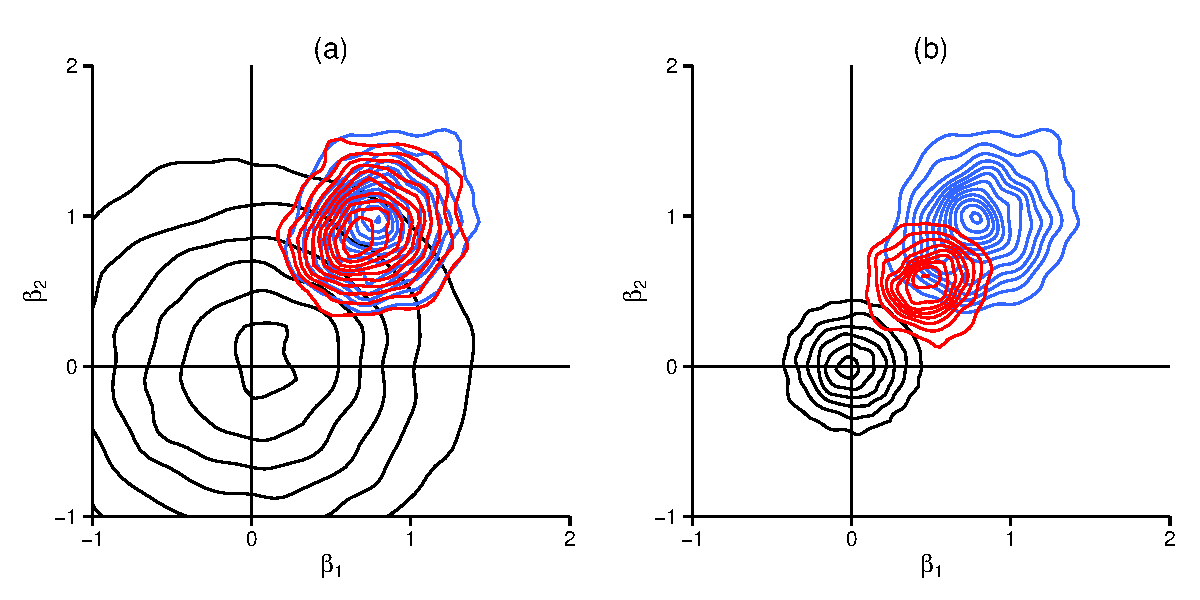
\includegraphics[width=0.8\textwidth]{prior_and_posterior}
%SHERMAN: Added "maximum likelihood estimator" "origin"
\caption{Illustration of the Bayesian logistic regression: the prior distribution (black), maximum likelihood estimator (blue), and posterior (red) shown by density plots in two different scenarios (a) and (b). Fixing $\beta_1=1$ and $\beta_2=1$, 100 data points were generated from the Bernoulli distribution with success probability $1/(1+\exp(-(\beta_1 x_1 + \beta_2 x_2)))$. The prior distribution is chosen as defined above with (a) $\lambda=0.01$ and (b) $\lambda=1$.}
\label{fig:prior_and_posterior}
\end{figure}

\subsection{Data augmentation scheme and Gibbs sampling}
 Sampling from the posterior distribution of $\boldbeta$ can be achieved by introducing the auxiliary random variables $\omega_i, i=1, ..., N$, and iterating the following two-step Gibbs sampling scheme:

\begin{enumerate}
\item $(\omega_i | \boldbeta) \sim \PG(1, x_i^T \boldbeta)$
\item $(\boldbeta | y, \omega) \sim \N(m_\omega, V_\omega)$
\end{enumerate}

where the first conditional distribution is a Polya-Gamma $PG(1, z)$ with some real number $z = x_i^T \boldbeta$ (see Figure~\ref{fig:proposed_naive} for examples), and the second one is a multivariate normal with the mean and covariance specified in \cite{polson2013bayesian}.
Note that there is a latent variable $\omega_i$ for each data point, i.e.~the first step needs to be implemented on each of the $N$ data points, whereas the parameters $\boldbeta$ are sampled jointly as a vector.

\begin{figure}[ht]
\centering
\centerline{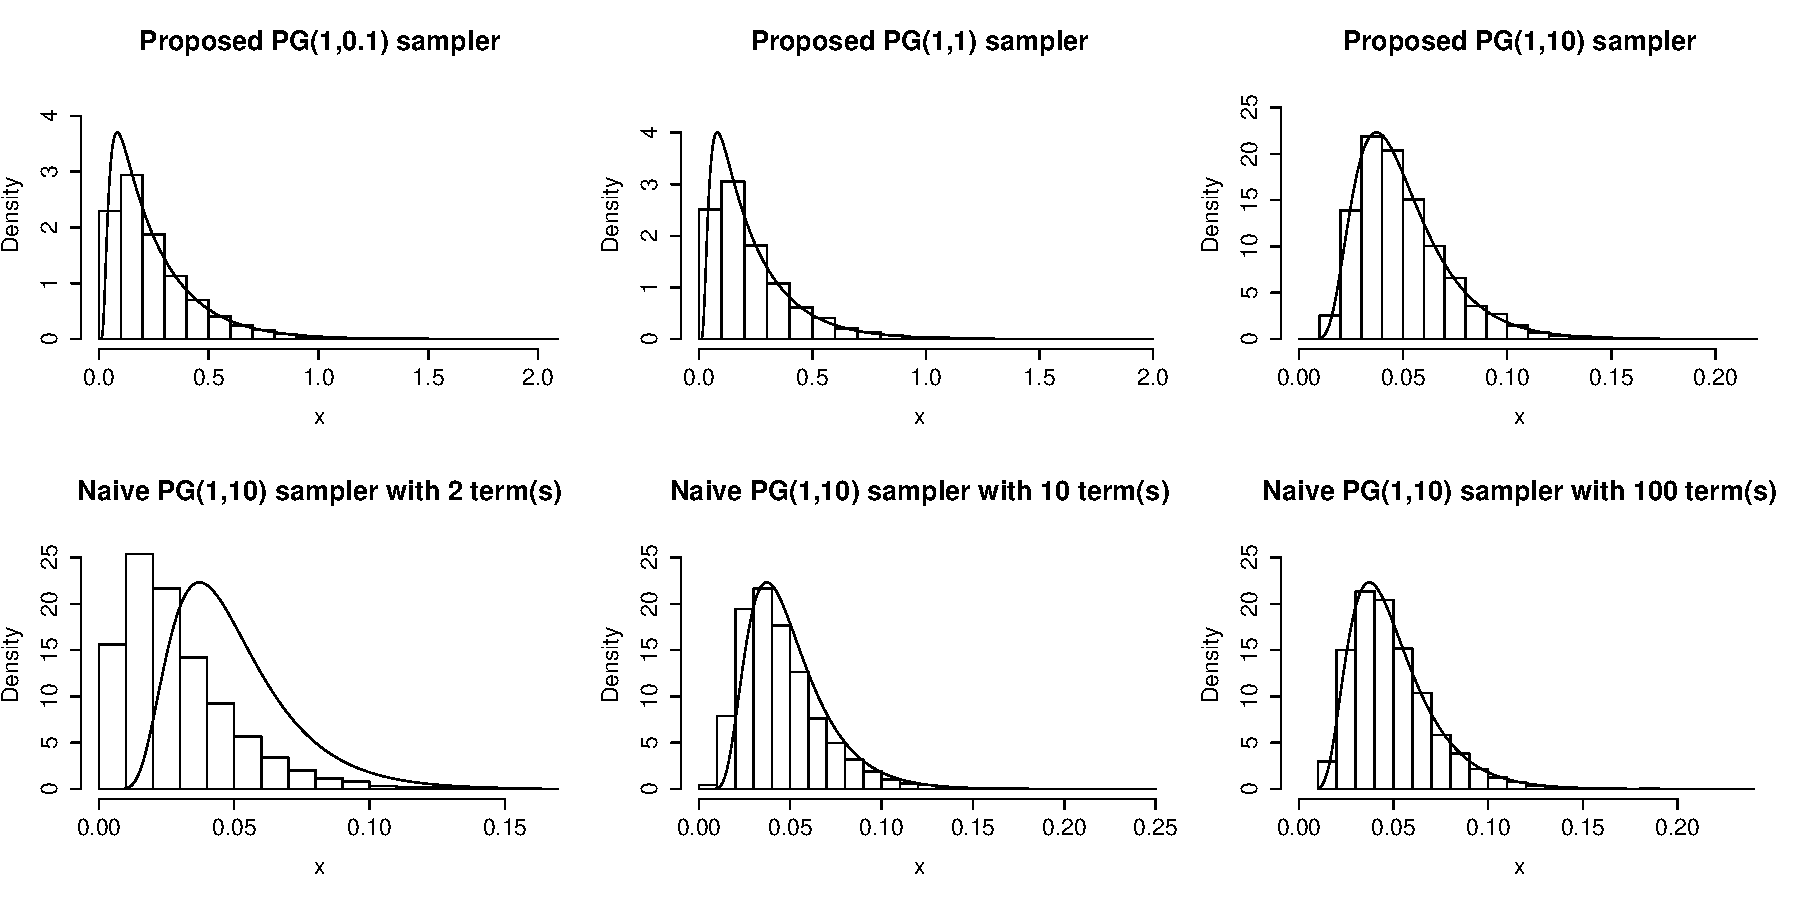
\includegraphics[width=1\textwidth]{proposed_naive}}
\caption{The 10,000 samples generated from the proposed (top row) and naive (bottom row) Polya-Gamma(1,$z$) sampler (histogram) plotted against the probability density function (curve).}
\label{fig:proposed_naive}
\end{figure}


One way for constructing a random variable $X$ from a Polya-Gamma distribution $PG(1, z)$ with $z \in \mathbb{R}$ was according to the definition, i.e.
\begin{equation} \label{PGdef}
\sum_{k=1}^\infty \frac{g_k}{(k-0.5)^2 + \frac{z^2}{4 \pi^2}}
\end{equation}
where $g_k \sim \Gamma(1, 1)$ are i.i.d.~random variables. The definition contains an infinite sum and it is not clear how its truncation to a finite number of terms will affect the results.

Instead, an accept-reject sampling procedure is proposed to sample from $PG(1,z)$.

\subsection{Sampling from the Polya-Gamma distribution}
Let $X\sim\textup{PG}(1,z)$, then the probability density function (p.d.f.) of $X$ is given as
\begin{equation}
f_X(x)=\sqrt{\frac{2}{\pi x^3}}\textup{cosh}\left(\dfrac{z}{2}\right)\exp{\left(-\frac{z^2x}{2}\right)}\sum_{n=0}^{\infty}\left(-1\right)^{-n}\left(n+1/2\right)\exp{\left[-\frac{(n+1/2)^2}{2x}\right]} \quad \textup{for }0<x.
\end{equation}
Rejection sampling on this p.d.f.~can be done by expressing it in a different form and in terms of the Jacobi distribution $\textup{J}^{*}(1,z)$. Suppose $J\sim \textup{J}^{*}(1,z/2)$ and has p.d.f.~$f_J(.)$, then the two distributions are related by $X=\frac{J}{4}$. As a result, samples from $J\sim\textup{J}^*(z/2)$ can be used to generate samples of $X\sim\textup{PG}(1,z)$.

The p.d.f.~of $J\sim \textup{J}^*(1,z)$ can be chosen to be expressed such that its partial sums have specific properties useful for rejection sampling. This can be done by setting the p.d.f.~of $J$ to be
\begin{equation}
f_J(x)=\textup{cosh}(z)\exp{\left(-\dfrac{xz^2}{2}\right)}\sum_{n=0}^{\infty}(-1)^n a_n(x) \quad \textup{for }0<x
\end{equation}
where the piecewise coefficients $a_n(x)$ are defined to be
\begin{equation}
a_n(x)=
\begin{cases}
\pi(n+1/2)\left(\dfrac{2}{\pi x}\right)^{3/2}\exp\left[-\dfrac{2(n+1/2)^2}{x}\right] & \text{ if } 0<x\leq  t\\[1em]
\pi(n+1/2)\exp\left[-\dfrac{(n+1/2)^2\pi^2x}{2}\right ]  & \text{ if } t<x
\end{cases}
\end{equation}
and $t=0.64$ is the truncation point. Let $S_r(x)$ be the partial sums such that
\begin{equation}
S_r(x)=\textup{cosh}(z)\exp{\left(-\dfrac{xz^2}{2}\right)}\sum_{n=0}^{r}(-1)^na_n(x) \ .
\end{equation}
A useful property of the partial sums is that they fluctuate around the target density symmetrically such that
\begin{equation}
S_0(x)>S_2(x)>\cdots>f_J(x)>\cdots>S_3(x)>S_1(x) \ .
\end{equation}
Because all $S_r(x)$ for even $r$ are bigger than the target distribution $f_J(x)$, $S_0(x)$ can be used as the proposal distribution where
\begin{equation}
S_0(x)=
\begin{cases}
\dfrac{\pi\textup{cosh}(z)}{2}\left(\dfrac{2}{\pi x}\right)^{3/2}\exp{\left(-\dfrac{xz^2}{2}-\dfrac{1}{2x}\right)} & \text{ if } 0<x\leq  t\\[1em]
\dfrac{\pi\textup{cosh}(z)}{2}\exp\left[-\left(\dfrac{z^2}{2}+\dfrac{\pi^2}{8}\right)x\right]  & \text{ if } t<x
\end{cases} \ .
\label{equation_s_0}
\end{equation}
Figure \ref{figure_sample_and_proposal} shows the density of the proposal (red and blue lines) and the target (black line) distribution together. They are indeed very close together and using such a proposal gives a very low rejection rate, no more than 9 rejections out of 10,000 samples, making it very efficient.

\begin{figure}[ht]
\centering
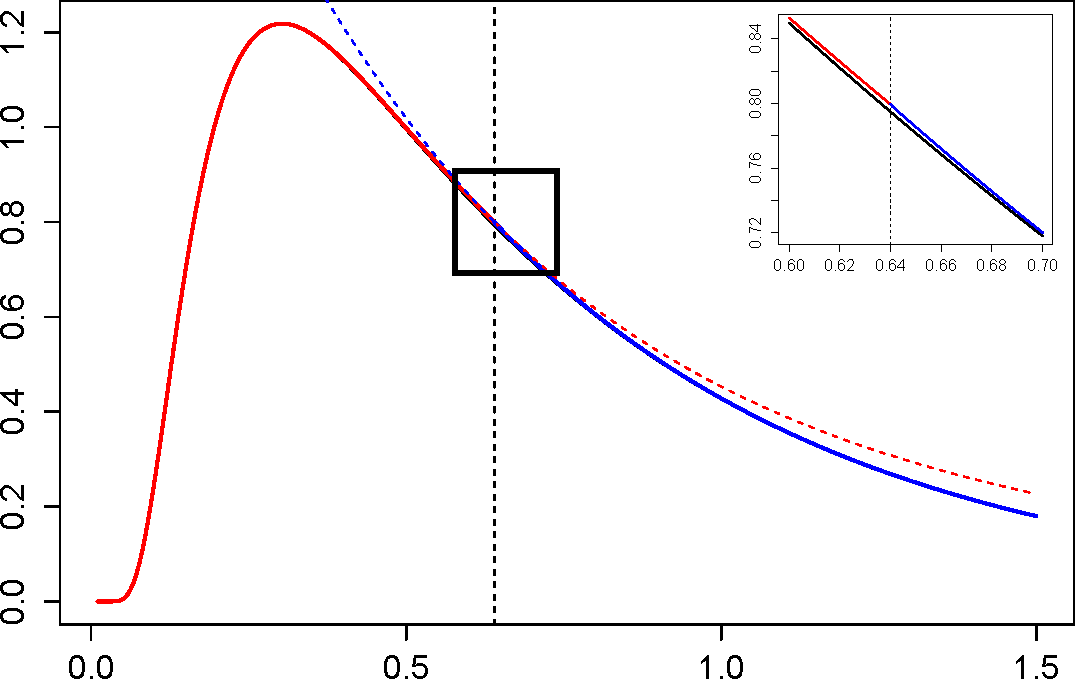
\includegraphics[width=0.6\textwidth]{fig_accept_reject_final}
\caption{Visualisation of the accept-reject algorithm for the target PG(1, 1) distribution (density in black). The proposal distribution is defined in two pieces: for $x \in (0, 0.64]$ (density in red) and $x \in (0.64, \infty)$ (blue). The middle portion of the figure has been zoomed in (top right corner). The dashed lines (red and blue) extend the densities of proposal distributions outside their defined range.}
\label{figure_sample_and_proposal}
\end{figure}

Examining equation \eqref{equation_s_0}, we can see that the first line corresponds to the density of the truncated Inverse Normal distribution and the bottom line to the truncated exponential distribution. Thus, denoting
\begin{align}
\Psi_1&\sim\textup{InverseNormal}(\left|z\right|^{-1},1) \\
\Psi_2&\sim\textup{Exp}(z^2/2+\pi^2/8)
\end{align}
the p.d.f. of the proposal $Y$ can be written as follows
\begin{equation}
f_Y(y)=\frac{1}{p+q}\left[
f_{\Psi_1}(y)\mathbb{I}_{0<y<t}+f_{\Psi_2}(y)\mathbb{I}_{y>t}
\right] \qquad \textup{for } 0<y \ ,
\end{equation}
where
\begin{equation}
p = \int_{0}^{t} f_{\Psi_1}(x) \textup{d}x \quad \textup{and} \quad
q = \int_{t}^{\infty} f_{\Psi_2}(x) \textup{d}x \ .
\end{equation}
This results in a relatively simple algorithm for sampling a random variable $Y$ from the proposal mixture.
\begin{itemize}
\item Generate $y$ from the proposal distribution $f_Y$, i.e.
  \begin{itemize}
  \item with probability $p/(p+q)$, sample $y$ from the truncated  $\textup{InverseNormal}(\left|z\right|^{-1},1)$
  \item with probability $q/(p+q)$ from the truncated $\textup{Exp}(z^2/2+\pi^2/8)$
  \end{itemize}
\item Apply the accept-reject approach. I.e.~generate $u\sim\textup{U}(0,y)$ and  accept this if $u<f(y)$, otherwise reject. Note that we cannot compute $f(y)$ exactly, we are comparing $u$ instead to the partial sums $S_r(y)$. If $u>S_r(y)$ for any even $r$, then $u>f_J(y)$ and the sample is rejected. Otherwise the sample is accepted if $u<S_r(y)$ for any odd $r$ as this implies $u<f_J(y)$.
\end{itemize}

% By examining Equation \ref{equation_s_0}, the proposal $Y$ can be sampled using a mixture model where
% \begin{align}
% \Psi_1&\sim\textup{InverseNormal}(\left|z\right|^{-1},1) \\
% \Psi_2&\sim\textup{Exp}(z^2/2+\pi^2/8)
% \end{align}
% and $Y$ has p.d.f.~
% \begin{equation}
% f_Y(y)=\frac{1}{p+q}\left[
% f_{\Psi_1}(y)\mathbb{I}_{0<y<t}+f_{\Psi_2}(y)\mathbb{I}_{y>t}
% \right] \qquad \textup{for } 0<y \ ,
% \end{equation}
% where
% \begin{equation}
% p = \int_{0}^{t} f_{\Psi_1}(x) \textup{d}x \quad \textup{and} \quad
% q = \int_{t}^{\infty} f_{\Psi_2}(x) \textup{d}x \ .
% \end{equation}
% In other words the proposal $Y$ can be sampled from the truncated $0<y<t$ $\textup{InverseNormal}(\left|z\right|^{-1},1)$ with probability $p/(p+q)$, and from the truncated $t<y$ $\textup{Exp}(z^2/2+\pi^2/8)$ with probability $q/(p+q)$.

% After obtaining a sample $y$ from the random variable $Y$, the accept-reject step was done by comparing the generated $U\sim\textup{U}(0,y)$ with the partial sums $S_r(y)$. If $U>S_r(y)$ for any even $r$, then $U>f_J(y)$ and the sample is rejected. Otherwise the sample is accepted if $U<S_r(y)$ for any odd $r$ as this implies $U<f_J(y)$.

\subsection{Example code}

Our implementation is available in PolyaGamma package within the function gibbs\_sampler. This can be used as follows

\begin{knitrout}
\definecolor{shadecolor}{rgb}{0.969, 0.969, 0.969}\color{fgcolor}\begin{kframe}
\begin{alltt}
\hlkwd{library}\hlstd{(PolyaGamma)}
\hlstd{data} \hlkwb{=} \hlkwd{generate_from_simple_logistic_model}\hlstd{(}\hlkwc{n}\hlstd{=}\hlnum{100}\hlstd{)}
\hlstd{obj} \hlkwb{=} \hlkwd{gibbs_sampler}\hlstd{(data}\hlopt{$}\hlstd{y, data}\hlopt{$}\hlstd{X,} \hlkwc{lambda}\hlstd{=}\hlnum{0.001}\hlstd{,} \hlkwc{n_iter_total}\hlstd{=}\hlnum{150}\hlstd{,} \hlkwc{burn_in}\hlstd{=}\hlnum{50}\hlstd{)}
\end{alltt}
\begin{verbatim}
## ===========================================================================
\end{verbatim}
\begin{alltt}
\hlstd{obj}
\end{alltt}
\begin{verbatim}
## 
##   MCMC sample from the posterior distribution of beta.
##   Chain length: 100 (with 50 burn-in removed).
##   Number of parameters: 2.
##   Posterior means: 1.674, 1.586.
##   Posterior standard deviations: 0.348, 0.429.
## 
\end{verbatim}
\end{kframe}
\end{knitrout}


\section{Experiments and results}

\subsection{Tests on simulated data}

As a proof of principle, we started by generating data from a simple logistic regression model, i.e.~with a success probability $P(y_i=1)$ modelled by $1/\exp(-(\beta_0 + \beta_1 x_i)))$. We have fixed $\beta_0 = 1$ and $\beta_1 = 1$ to generate samples of varying size $N$. For all the following analysis we run the MCMC chain for 500 iterations and discarded the first 100 as burn-in.

Trace plots (Figure \ref{fig:traceplot}) indicate good mixing of the chains and the autocorrelations are relatively small. On the simple example the sampler seems to work efficiently.
Next, we verified that for increasing sample size $N$, the posterior distribution of the parameter becomes more and more concentrated towards the true value (boxplots and the decreasing mean squared error in Figure \ref{fig:posterior_and_mse} indicate this). Additionally, we verified the correctness of our implementation by estimating the posterior distributions with the BayesLogit package and comparing the results. As expected, these are highly similar, with small deviations likely arising from a different initialisation.

\begin{figure}[ht]
\centering
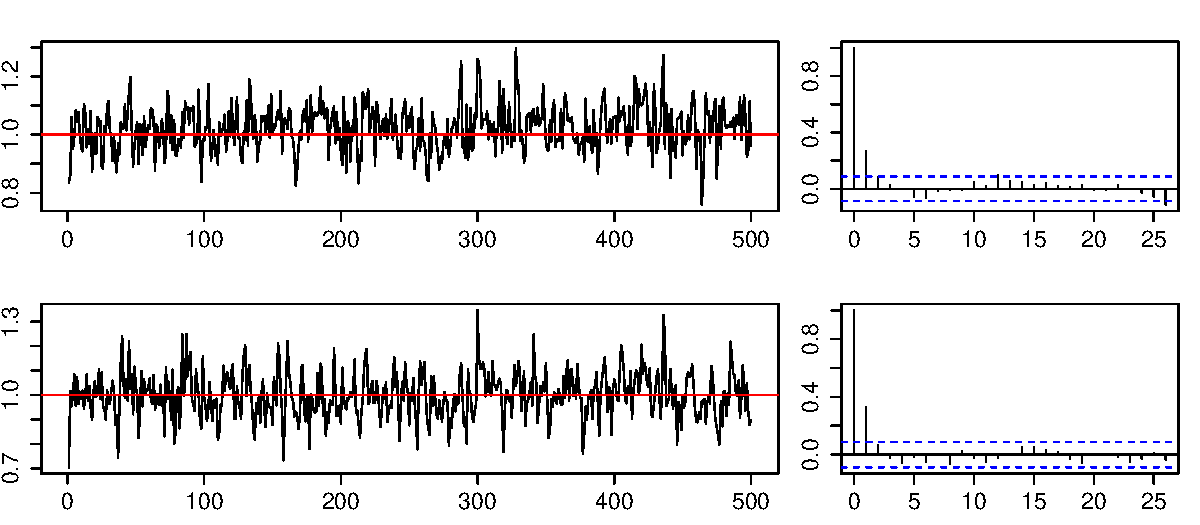
\includegraphics[width=0.8\textwidth]{fig_traceplot_beta}
\caption{Traceplot (left) and autocorrelations (right) from the chains of $\beta_0$ (top row) and $\beta_1$ (bottom row) on simulated data. Horizontal red line denotes the true value. }
\label{fig:traceplot}
\end{figure}


\begin{figure}[ht]
\centering
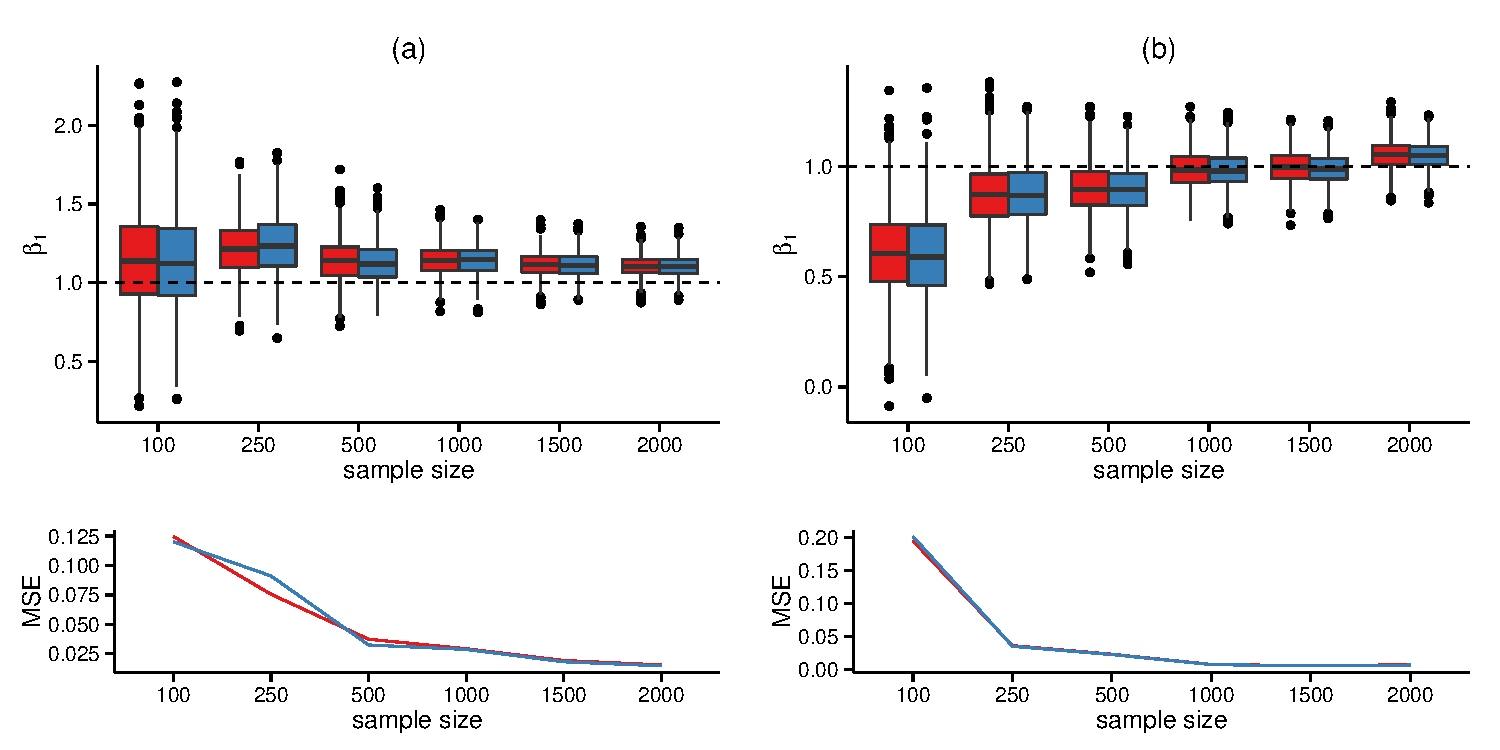
\includegraphics[width=\textwidth]{posterior_and_mse}
\caption{Samples from the posterior distribution of the parameter, comparing our implementation (red) and the BayesLogit package (blue), for a vague prior (a) $\lambda=0.01$ and a strong one (b) $\lambda=10$.}
\label{fig:posterior_and_mse}
\end{figure}


\subsection{Tests on real data}

Experiments were conducted to investigate how the Bayesian logistic regression can be used as a classifier on real datasets. The classifier was then compared, in prediction error, with the classical logistic regression.

Each dataset was randomly split into two equally sized disjoint subsets, the training and test set. The classifier was trained using the training set, and the training set only, so that it can be used to predict the responses given the feature vectors. The prior, used in the experiments, was set to be as non-informative as possible but can be varied univariately by changing $\lambda$.
Because the precision matrix is a diagonal matrix with equal entries, the training sets were normalised to have zero mean and standard deviation of one, this was done so that the prior has an equal impact on all elements of the posterior $\boldbeta$. The predictive distribution, given a feature vector $x$, is the posterior expectation of the likelihood, that is
\begin{equation}
\textup{E}_{\boldbeta|\mathbf{Y}}\left[\dfrac{1}{1+\textup{e}^{- x^\textup{T}\boldbeta}}\right] \ .
\end{equation}
Prediction of the response variable, given the feature vector $x$, was done by estimating the posterior expectation of the likelihood by taking a sample mean of the logistic function. %using 400 posterior samples of $\boldbeta$ from the Gibbs sampler, after 100 iterations for burning in.
In other words, after obtaining the samples $\boldbeta_1,\boldbeta_2,\cdots,\boldbeta_{M}$ from the posterior distribution, the prediction of the response $\widehat{y}$, given the feature vector $x$, is
\begin{equation}
\widehat{y}=\textup{round}\left[\sum_{i=1}^{M}\dfrac{1}{1+\textup{e}^{- x^\textup{T}\boldbeta_i}}\right] \ .
\end{equation}
As stated before, we used $M=400$. This was repeated 5 times to get a sample of training and test errors.

Two datasets were investigated in the experiment. \emph{SAheart} is a small dataset with sample size $N=462$ and number of features (including an intercept) $p=7$, while \emph{spambase} is a large dataset with $N=4601$ and $p=58$. Figures \ref{fig:sa_heart} and \ref{fig:spambase} shows the training and test errors of the two datasets. With regards to \emph{SAheart}, as expected the training error decreased for smaller, and less informative, prior precision. For $\lambda=10^{2}$, the test error showed evidence that the Bayesian logistic regression outperforms the classical logistic regression. For the dataset \emph{spambase}, the training error behaved as expected with smaller prior precision giving smaller training errors. However for this dataset, on average the test errors are larger compared to the results obtained from classical logistic regression.

The performance of the Bayesian logistic regression compared with the classical version were similar and may be better depending on the dataset. Nevertheless, Bayesian logistic regression may be a good candidate for a binary classifier, where selecting the value of $\lambda$ which optimises the test error may be done by using cross validation methods.

\begin{figure}
    \centerline{\centering
    \begin{subfigure}[b]{0.6\textwidth}
        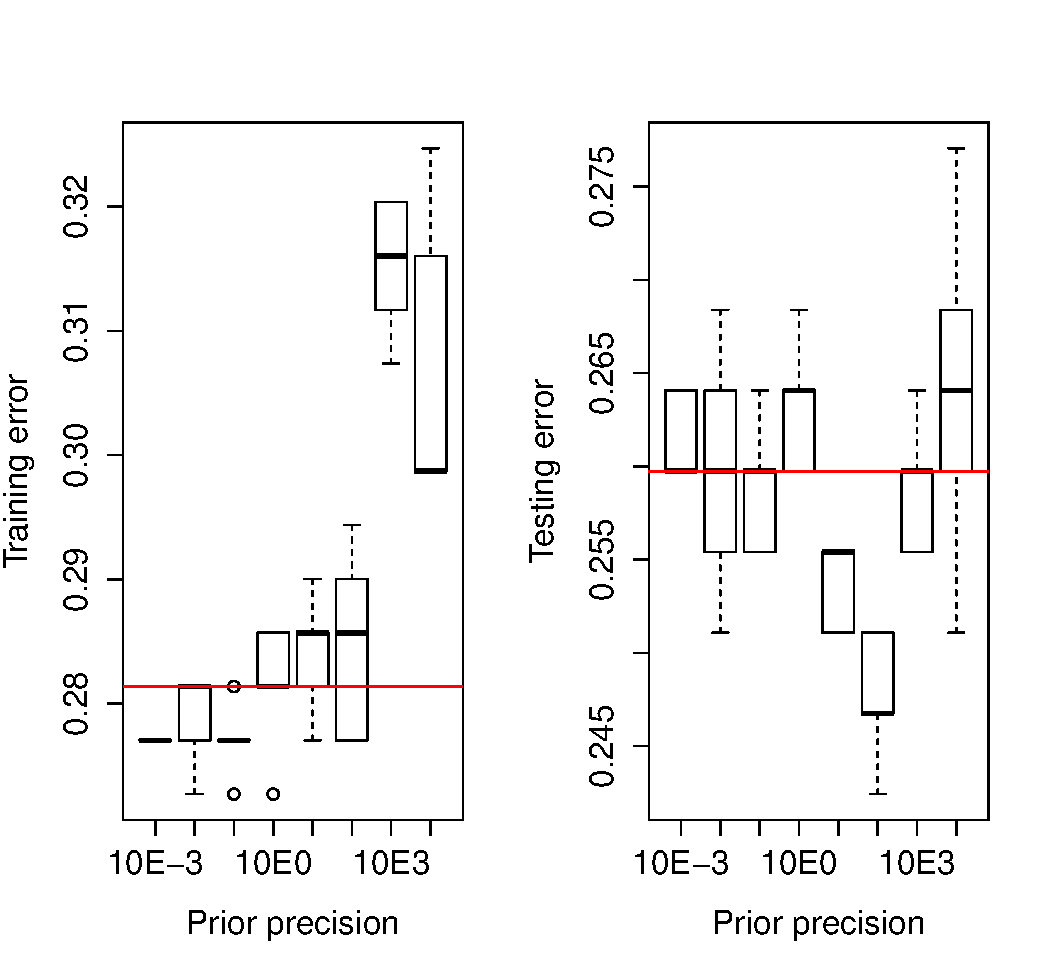
\includegraphics[width=\textwidth]{sa_heart}
        \caption{\emph{SAheart}}
        \label{fig:sa_heart}
    \end{subfigure}
    \begin{subfigure}[b]{0.6\textwidth}
        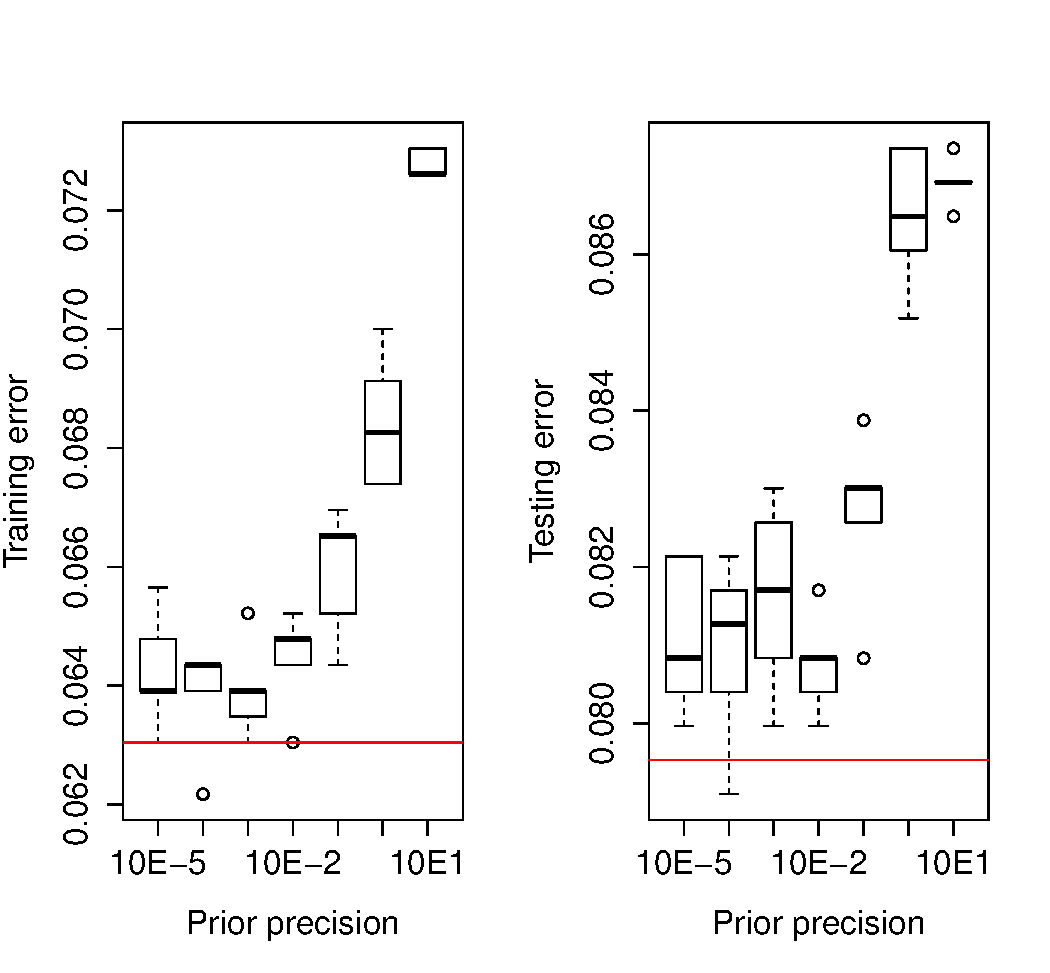
\includegraphics[width=\textwidth]{spambase}
        \caption{\emph{spambase}}
        \label{fig:spambase}
    \end{subfigure}}
    \caption{Training and testing error on the dataset \emph{SAheart} and \emph{spambase} using the Bayesian logistic regression (box plot) and classical logistic regression (red line). The Bayesian logistic regression made predictions by using the sample mean of 400 posterior logistic regressions, this was repeated 5 times to get a sample of errors on the training and test set.}\label{fig:animals}
\end{figure}

\subsection{Naive sampler for Polya-Gamma distribution}

Instead of using the accept-reject method proposed in \cite{polson2013bayesian}, in principle one could simply truncate the infinite sum in \eqref{PGdef}. Thus we compared this naive approach with the more extensive simulation.

With a small (ten or smaller) number of terms, the truncated sum is not a good approximation of the Polya-Gamma distribution (Figure~\ref{fig:proposed_naive}), but using 100 terms approximates the Polya-Gamma density quite well.
Carrying out comparison of average computation time, we saw that compared to the proper accept-reject simulation, the approximation of 100 terms is four times faster.

We applied both the naive sampler and the proposed sampler to the real data sets, and compared the test error. For a fixed $\lambda=0.001$, the results were comparable, whereas the naive approach provided slightly less accurate out-of-sample predictions. The test errors for \emph{SAheart} data were 0.26 and 0.27 (exact vs. naive), and for \emph{spambase} data 0.08 and 0.11 (exact vs naive). For the latter, we observed problems with the convergence of the chains, see an example in Figure~\ref{fig:naive_convergence}.

\begin{figure}[!htbp]
\centering
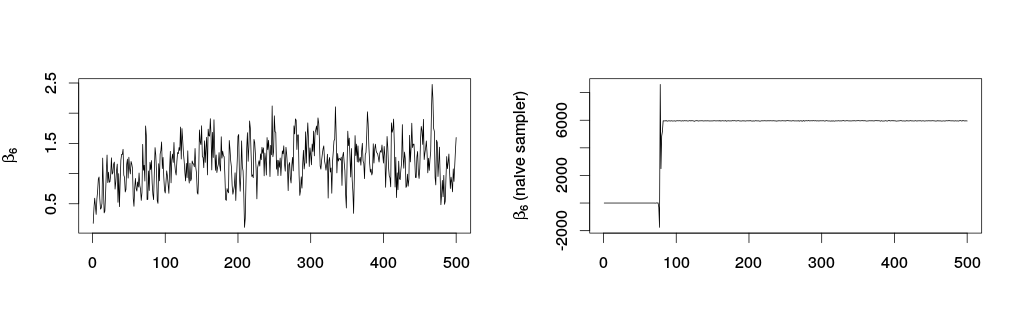
\includegraphics[width=\textwidth]{naive_sampler}
\caption{Naive Polya-Gamma sampler may produce a chain which converges to widely different values. Traceplot for the first 500 iterations for parameter $\beta_6$ from the spambase data, using either the proposed sampler (left) or the naive one (right). }
\label{fig:naive_convergence}
\end{figure}

\subsection{Comparison with BayesLogit package}

In section 3.1, we verified that our implementation provides highly similar posterior distribution as the BayesLogit package. Next, we compared the performance of our implementation with the one provided in BayesLogit package. Their approach is slightly different from ours, as they bin the data according to the features $x_i$, and aggregate the binary $y_i$ values  for each unique $x_i$. We note that this may reduce the number of latent variables $\omega_i$.

The respective computation times over 5 repetitions are shown in Table \ref{tab:comptime}. As BayesLogit package uses C calls, it is remarkably faster compared to our implementation (on the large \emph{spambase} dataset, the average computation time 2 seconds versus 63 seconds). Using a naive Polya-Gamma sampler reduces computation time compared to our implementation of the proposed sampler, but as shown previously (Fig. \ref{fig:naive_convergence}), this approximation may be unreliable.

\begin{table}[!htbp]
\centering
\caption{Computation time in seconds for the two data sets studied. Chains were run for 500 iterations.}
\label{tab:comptime}
\begin{tabular}{rrrrrrr}
  \hline
  & \multicolumn{3}{c}{SAheart} & \multicolumn{3}{c}{spambase} \\
 & min & mean & max & min & mean & max \\
  \hline
BayesLogit & 0.06 & 0.06 & 0.07 & 1.64 & 1.69 & 1.71 \\
Our implementation (naive) & 1.50 & 1.55 & 1.65 & 19.42 & 19.61 & 19.78 \\
Our implementation & 5.50 & 5.56 & 5.60 & 62.95 & 63.25 & 63.70 \\
   \hline
\end{tabular}
\end{table}


\bibliographystyle{plainnat}
\bibliography{mybib}

\end{document}
